\documentclass{article}

% Import necessary packages
\usepackage{amsmath}
\usepackage{amssymb}
\usepackage{graphicx}
\usepackage{hyperref}
\usepackage{listings}
\usepackage{xcolor}
\usepackage{braket}
% Set page margins
\usepackage[margin=1in]{geometry}

% Set code block style
\lstset{
    basicstyle=\ttfamily,
    keywordstyle=\color{blue},
    commentstyle=\color{gray},
    stringstyle=\color{purple},
    showstringspaces=false,
    breaklines=true,
    breakatwhitespace=true,
    captionpos=b,
    frame=single,
    numbers=left,
    numbersep=5pt,
    numberstyle=\tiny\color{gray},
    backgroundcolor=\color{lightgray!20},
    rulecolor=\color{black},
    tabsize=4
}

% Set title and author
\title{Assignment 2}
\author{Wang Dingrui}

\begin{document}

\maketitle

\section{EXERCISE 1: THE PARTIAL TRACE}

We saw in the lectures that given a multi-partite state, we obtain the state of a subsystem by applying the partial trace to the other systems.

\begin{enumerate}
    \item Compute the trace of the following states by applying the trace formula $ Tr(A)=\sum_i\bra{i}A\ket{i} $ from the lectures:
          \begin{enumerate}
              \item $\xi = \frac{1}{2}(\ket{0}\bra{0} - i\ket{0}\bra{1} + i\ket{1}\bra{0} + \ket{1}\bra{1})$
              \item $\Lambda = \frac{I}{3}I + \frac{1}{6}(\ket{0}\bra{1} + \ket{1}\bra{0})$ (here, $I$ is the identity matrix).

                    Which of the states is normalized correctly? (*) (4 points)
          \end{enumerate}
          Answer: $\xi = \frac{1}{2}(\ket{0}\bra{0} - i\ket{0}\bra{1} + i\ket{1}\bra{0} + \ket{1}\bra{1})$

          $Tr(\xi) = \bra{0}\xi\ket{0}+\bra{1}\xi\ket{1}
              =\frac{1}{2}(\braket{0|0}\braket{0|0}-i\braket{text|0}\braket{1|0}+i\braket{0|1}\braket{0|0}+\braket{0|1}\braket{1|0}
              +\braket{1|0}\braket{0|1}-i\braket{1|0}\braket{1|1}+i\braket{1|1}\braket{0|1}+\braket{1|1}\braket{1|1})
              =\frac{1}{2}(1+1)
              =1
          $

          $\Lambda = \frac{I}{3}I + \frac{1}{6}(\ket{0}\bra{1} + \ket{1}\bra{0})
              =\frac{1}{3}\ket{0}\bra{0}+\frac{1}{6}\ket{0}\bra{1}+\frac{1}{6}\ket{1}\bra{0}+\frac{1}{3}\ket{1}\bra{1}
          $


          $Tr(\Lambda) = \bra{0}\Lambda\ket{0}+\bra{1}\Lambda\ket{1}
              \\=\frac{1}{3}\braket{0|0}\braket{0|0}+\frac{1}{6}\braket{0|0}\braket{1|0}+\frac{1}{6}\braket{0|1}\braket{0|0}+\frac{1}{3}\braket{0|1}\braket{1|0}
              +\frac{1}{3}\braket{1|0}\braket{0|1}+\frac{1}{6}\braket{1|0}\braket{1|1}+\frac{1}{6}\braket{1|1}\braket{0|1}+\frac{1}{3}\braket{1|1}\braket{1|1}
              \\=\frac{1}{3}(1+1)
              \\=\frac{2}{3}
          $

          So $\xi$ is normalized correctly.


    \item In the last assignment we found the probability to find a state $\ket{\gamma}$ in another state $\ket{\delta}$ to be $p = |\braket{\gamma|\delta}|^2$. Show here that this expression coincides with $\mathrm{Tr}(\gamma\delta)$, for $\gamma = \ket{\gamma}\bra{\gamma}$ and $\delta = \ket{\delta}\bra{\delta}$. Hint: Apply the trace formula $\mathrm{Tr}(A) = \sum_i \braket{i|A|i}$ from the lectures. Use a suitable basis of your choice. (4 points)

          Answer:

          Assume $\ket{\gamma}=\alpha_0\ket{0}+\alpha_1\ket{1}$ and $\ket{\delta}=\beta_0\ket{0}+\beta_1\ket{1}$


          $\braket{\gamma|\delta}=\alpha_0^*\beta_0+\alpha_1^*\beta_1$


          $\mathrm{Tr}(\gamma\delta)
              \\= \mathrm{Tr}(\ket{\gamma}\bra{\gamma}\ket{\delta}\bra{\delta})
              \\= \mathrm{Tr}(\ket{\gamma}\braket{\gamma|\delta}\bra{\delta})
              \\= \mathrm{Tr}(\braket{\gamma|\delta}\ket{\gamma}\bra{\delta})
              \\= \braket{\gamma|\delta}\mathrm{Tr}(\ket{\gamma}\bra{\delta})
              \\= \braket{\gamma|\delta}\sum_i\braket{i|\ket{\gamma}\bra{\delta}|i}
              \\= \braket{\gamma|\delta}(\bra{0}\ket{\gamma}\bra{\delta}\ket{0}+\bra{1}\ket{\gamma}\bra{\delta}\ket{1})
              \\= \braket{\gamma|\delta}(\braket{0|\gamma}\braket{\delta|0}+\braket{1|\gamma}\braket{\delta|1})
              \\= \braket{\gamma|\delta}(\alpha_0^*\beta_0+\alpha_1^*\beta_1)
              \\= (\alpha_0^*\beta_0+\alpha_1^*\beta_1)(\alpha_0^*\beta_0+\alpha_1^*\beta_1)
              \\= (\alpha_0^*\beta_0+\alpha_1^*\beta_1)^2
              \\=|\braket{\gamma|\delta}|^2$

          So, $\mathrm{Tr}(\gamma\delta) = |\braket{\gamma|\delta}|^2 = p$.

    \item Consider the bipartite state $\ket{\phi}_{AB} = \frac{1}{\sqrt{3}}(\ket{00}_{AB} + i\ket{01}_{AB} - \ket{11}_{AB})$. Write the density operator $\rho_{AB} = \ket{\phi}_{AB}\bra{\phi}_{AB}$ explicitly in matrix form. (*) (4 points)

          Answer:
          $\phi_{AB}=\frac{1}{\sqrt{3}}(\ket{00}_{AB} + i\ket{01}_{AB} - \ket{11}_{AB})
              \\=\frac{1}{\sqrt{3}}(
              \begin{bmatrix}
                  1 \\ 0 \\ 0 \\ 0 \\
              \end{bmatrix}
              +i\begin{bmatrix}
                  0 \\ 1 \\ 0 \\ 0 \\
              \end{bmatrix}
              -\begin{bmatrix}
                  0 \\ 0 \\ 0 \\ 1 \\
              \end{bmatrix})
              \\=\frac{1}{\sqrt{3}}\begin{bmatrix}
                  1 \\ i \\ 0 \\ -1 \\
              \end{bmatrix}
          $

          $\rho_{AB}
              \\= \ket{\phi}_{AB}\bra{\phi}_{AB}
              \\=\frac{1}{3}\begin{bmatrix}
                  1 \\ i \\ 0 \\ -1 \\
              \end{bmatrix}\begin{bmatrix}
                  1 & -i & 0 & -1 \\
              \end{bmatrix}
              \\=\frac{1}{3}\begin{bmatrix}
                  1  & -i & 0 & -1 \\
                  i  & 1  & 0 & -i \\
                  0  & 0  & 0 & 0  \\
                  -1 & -i & 0 & 1  \\
              \end{bmatrix}
              \\= \begin{bmatrix}
                  \frac{1}{3}  & -\frac{i}{3} & 0 & -\frac{1}{3} \\
                  \frac{i}{3}  & \frac{1}{3}  & 0 & -\frac{i}{3} \\
                  0            & 0            & 0 & 0            \\
                  -\frac{1}{3} & \frac{i}{3}  & 0 & \frac{1}{3}  \\
              \end{bmatrix}
          $

    \item Let $\sigma_{AB}$ be a general 2-qubit state. The $4\times4$ matrix describing $\sigma_{AB}$ can be split into four sub-matrices of size $2\times2$ (upper left block, upper right block, lower left block, lower right block). Show that the reduced single qubit state $\sigma_B = \mathrm{Tr}_A(\sigma_{AB})$ is described by a $2\times2$ matrix that is the sum of the upper left block and lower right block matrices of $\sigma_{AB}$. Hint: start from $\sigma_{AB} = \sigma_{00}|00\rangle\langle00| + \sigma_{01}|00\rangle\langle01| + ... + \sigma_{33}|11\rangle\langle11|$ and compute the partial trace in bra-ket notation. Write $\sigma_{AB}$ as a matrix and compare. (8 points)

          Answer: $\sigma_{AB} = \sigma_{00}\ket{00}\bra{00} + \sigma_{01}\ket{00}\bra{01} + ... + \sigma_{33}\ket{11}\bra{11}$


          $\sigma_B =
              \\=\mathrm{Tr}_A(\sigma_{AB})
              \\= \sum_i\bra{i}_A\sigma_{AB}\ket{i}_A
              \\= \bra{0}_A\sigma_{AB}\ket{0}_A+\bra{1}_A\sigma_{AB}\ket{1}_A
              \\= \bra{0}_A(\sigma_{00}\ket{00}_{AB}\bra{00} + \sigma_{01}\ket{00}_{AB}\bra{01}_{AB} + ... + \sigma_{33}\ket{11}_{AB}\bra{11}_{AB})\ket{0}+\bra{1}(\sigma_{00}\ket{00}_{AB}\bra{00}_{AB} + \sigma_{01}\ket{00}_{AB}\bra{01}_{AB} + ... + \sigma_{33}\ket{11}_{AB}\bra{11}_{AB})\ket{1}_A
              \\=\sigma_{00}\ket{0}\bra{0}+\sigma_{01}\ket{0}\bra{1}+\sigma_{10}\ket{1}\bra{0}+\sigma_{11}\ket{1}\bra{1}+\sigma_{22}\ket{0}\bra{0}+\sigma_{23}\ket{0}\bra{1}+\sigma_{32}\ket{1}\bra{0}+\sigma_{33}\ket{1}\bra{1}
              \\=(\sigma_{00}+\sigma_{22})\ket{0}\bra{0}+(\sigma_{01}+\sigma_{23})\ket{0}\bra{1}+(\sigma_{10}+\sigma_{32})\ket{1}\bra{0}+(\sigma_{12}+\sigma_{33})\ket{1}\bra{1}
          $

          This is the sum of the upper left block and lower right block matrices of $\sigma_{AB}$.

    \item Take the state $\rho_{AB}$ from 3. and compute the reduced state $\rho_B$, both from the matrix itself (using your result from 4.) and in bra-ket notation. (*) (6 points)

          Answer: $\begin{bmatrix}
                  \frac{1}{3}  & -\frac{i}{3} & 0 & -\frac{1}{3} \\
                  \frac{i}{3}  & \frac{1}{3}  & 0 & -\frac{i}{3} \\
                  0            & 0            & 0 & 0            \\
                  -\frac{1}{3} & \frac{i}{3}  & 0 & \frac{1}{3}  \\
              \end{bmatrix}$

          $\rho_B = (\sigma_{00}+\sigma_{22})\ket{0}\bra{0}+(\sigma_{01}+\sigma_{23})\ket{0}\bra{1}+(\sigma_{10}+\sigma_{32})\ket{1}\bra{0}+(\sigma_{12}+\sigma_{33})\ket{1}\bra{1}
              \\= \frac{1}{3}\ket{0}\bra{0}-\frac{i}{3}\ket{0}\bra{1}+\frac{i}{3}\ket{1}\bra{0}+0\ket{1}\bra{1}
              \\= \begin{bmatrix}
                  \frac{1}{3} & -\frac{i}{3} \\
                  \frac{i}{3} & \frac{2}{3}  \\
              \end{bmatrix}$
\end{enumerate}

\section{EXERCISE 2: MEASUREMENTS AND REDUCED STATES}
Let us look at the density operator $\rho_{AB} = |\Phi^{-}\rangle\langle\Phi^{-}|$, with $|\Phi^{-}\rangle = \frac{1}{\sqrt{2}}(\ket{01} - \ket{10})$.

\begin{enumerate}
    \item Compute explicitly the post-measurement state after we performed a projective measurement $M = \{\ket{0}\bra{0},\ket{1}\bra{1}\}$ on $\rho_{AB}$ on system $B$, given that the outcome was $0$. Compute the same for the measurement $M = \{|+\rangle\langle+|, |-\rangle\langle-|\}$, for outcome $-$. (Hint: Using Exercise 2.6 from Assignment 1 might help (not necessary though).) (8 points)

          Answer: $M_0=\ket{0}\bra{0}$

          Observe $\ket{0}$ with probability $p_0=Tr(M_0\rho)=Tr(I\otimes \ket{0}\bra{0}\rho)=Tr(I\otimes \ket{0}\bra{0}\ket{\Phi^{-}}\bra{\Phi^{-}})=Tr(I\otimes \ket{0}\bra{0}\frac{1}{2}(\ket{01}\bra{10}-\ket{01}\bra{01}-\ket{10}\bra{10}+\ket{10}\bra{01}))=Tr(\frac{1}{2}(-\ket{10}\bra{10}+\ket{10}\bra{01}))=-\frac{1}{2}$

          $\rho_0'=\frac{M_0\rho M_0^{\dagger}}{Tr(M_0\rho)}
              \\=\frac{I\otimes \ket{0}\bra{0}\ket{\Phi^{-}}\bra{\Phi^{-}}I\otimes \ket{0}\bra{0}}{Tr(\frac{1}{2}(-\ket{10}\bra{10}+\ket{10}\bra{01}))}
              \\=\frac{\frac{1}{2}(-\ket{10}\bra{10}+\ket{10}\bra{01})I\otimes \ket{0}\bra{0}}{-\frac{1}{2}}
              \\=\ket{10}\bra{10}
          $

          For system B, $\rho_{0B}'=\ket{0}\bra{0}$


          $M_1=\ket{-}\bra{-}$

          Observe $\ket{-}$ with probability $p_1=Tr(M_1\rho)=Tr(I\otimes \ket{-}\bra{-}\rho)=Tr(I\otimes \ket{-}\bra{-}\ket{\Phi^{-}}\bra{\Phi^{-}})=
              Tr(I\otimes \ket{-}\bra{+}\frac{1}{2}(\ket{+-}\bra{-+}-\ket{+-}\bra{+-}-\ket{-+}\bra{-+}+\ket{-+}\bra{+-}))
              \\=\frac{1}{2}Tr(\ket{+-}\bra{-+}-\ket{+-}\bra{+-})=-\frac{1}{2}
          $

          $\rho_1'=\frac{M_1\rho M_1^{\dagger}}{Tr(M_1\rho)}
              \\=\frac{(\ket{+-}\bra{-+}-\ket{+-}\bra{+-})I\otimes \ket{-}\bra{-}}{\bra{+}\otimes I\ket{\Phi^-}\bra{\Phi^-}\ket{+}\otimes I}
              \\=\ket{+-}\bra{+-}
              \\=\ket{+}\bra{-}\otimes\ket{+}\bra{-}
          $

          For system B, $\rho_{1B}'=\ket{-}\bra{-}$

    \item What is the post measurement state if the measurements above were destructive and yielded the same outcomes as in part 1.? (2 points)

          Answer:

          For the outcome 0, $\rho_0''=\frac{M_0\rho_{0}'M_0^\dagger}{Tr(M_0\rho_{0})}=\frac{M_0\ket{10}\bra{10}M_0^\dagger}{Tr(M_0\ket{10}\bra{10})}=\frac{I\otimes\ket{0}\bra{0}\ket{10}\bra{10}I\otimes\ket{0}\bra{0}}{Tr(I\otimes\ket{0}\bra{0}\ket{10}\bra{10})}=\ket{10}\bra{10}$


          For the outcome -, $\rho_-''=\frac{M_1\rho_{1}'M_1^\dagger}{Tr(M_1\rho_{1})}=\frac{M_1\ket{+-}\bra{+-}M_1^\dagger}{Tr(M_1\ket{+-}\bra{+-})}=\frac{I\otimes\ket{-}\bra{-}\ket{+-}\bra{+-}I\otimes\ket{-}\bra{-}}{Tr(I\otimes\ket{-}\bra{-}\ket{+-}\bra{+-})}=\ket{+-}\bra{+-}$

    \item What is the reduced state $\rho_A$ if we take state $\rho_{AB}$ and trace over system B in basis $\{\ket{0}, \ket{1}\}$? What if we trace in $\{\ket{+}, \ket{-}\}$? Hint: for the second computation it could be useful to use the basis invariance of the trace operation. (6 points)

          Answer: $\rho_{AB}=\ket{\Phi^-}\bra{\Phi^-}=\frac{1}{2}(\ket{01}-\ket{10})(\bra{10}-\bra{01})
              =\frac{1}{2}(\ket{01}\bra{10}-\ket{01}\bra{01}-\ket{10}\bra{10}+\ket{10}\bra{01})
          $


          $\rho_A=Tr_B(\rho_{AB})=\bra{0}_B\rho_{AB}\ket{0}_B+\bra{1}_B\rho_{AB}\ket{1}_B=-\frac{1}{2}\ket{0}\bra{0}-\frac{1}{2}\ket{1}\bra{1}
          $


          In the basis $\{\ket{+},\ket{-}\}$, $\Phi=\frac{1}{2}(\ket{+}\otimes\ket{-}-\ket{-}\otimes\ket{+})$

          $\rho_A=Tr_B(\rho_{AB})=\bra{+}_B\rho_{AB}\ket{+}_B+\bra{-}_B\rho_{AB}\ket{-}_B
              \\=\frac{1}{2}((\bra{0}_B+\bra{1}_B)\rho_{AB}(\ket{0}_B+\ket{1}_B))+\frac{1}{2}((\bra{0}_B-\bra{1}_B)\rho_{AB}(\ket{0}_B-\ket{1}_B))
              \\=\frac{1}{2}(\bra{0}_B\rho_{AB}\ket{0}_B+\bra{0}_B\rho_{AB}\ket{1}_B+\bra{1}_B\rho_{AB}\ket{0}_B+\bra{1}_B\rho_{AB}\ket{1}_B+\bra{0}_B\rho_{AB}\ket{0}_B-\bra{0}_B\rho_{AB}\ket{1}_B-\bra{1}_B\rho_{AB}\ket{0}_B+\bra{1}_B\rho_{AB}\ket{1}_B)
              \\=\frac{1}{2}(2\bra{0}_B\rho_{AB}\ket{0}_B+2\bra{1}_B\rho_{AB}\ket{1}_B)
              \\=\bra{0}_B\rho_{AB}\ket{0}_B+\bra{1}_B\rho_{AB}\ket{1}_B
              \\=-\frac{1}{2}\ket{0}\bra{0}-\frac{1}{2}\ket{1}\bra{1}
          $

    \item Consider now the $2n$-qubit state $\rho = \ket{\Psi_n}\bra{\Psi_n}$, with $\ket{\Psi_n} = \frac{1}{\sqrt{2^n}}\sum_i \ket{i}_A \otimes \ket{i}_B$. What is the reduced $n$-qubit state on Alice's side? (Hint: look at the state in vector form and factorize it in a smart way.) (8 points)


          Answer: $\rho=\frac{1}{2^n}\sum_i\ket{i}_A\otimes \ket{i}_B\bra{i}_A\bra{i}_B
              \\=\frac{1}{2^n}\sum_i\ket{i}_A\otimes\ket{i}_B\bra{i}_A\otimes\bra{i}_B
          $

          $Tr_B(\rho)=\frac{1}{2^n}\sum_k\sum_i\bra{k}\ket{i}\bra{i}\otimes\ket{i}\bra{i}\ket{k}$

          If $i\neq k$, $\bra{k}\ket{i}=0$


          $Tr_B(\rho)=\frac{1}{2^n}\sum_i\bra{i}\ket{i}\otimes\ket{i}\bra{i}\otimes\bra{i}\ket{i}
              \\=\frac{1}{2^n}\sum_i\ket{i}\bra{i}
              \\=\frac{I_n}{2^n}
          $
    \item What is the reduced state on the first $k$ qubits of A and B (i.e. tracing out the last $n - k$ qubits on each side)?(4 points)

          Answer: $\rho_{0 \to k-1} = Tr_{\rho_{k \to n-1}}(\rho_{AB}) = \sum_{m=k}^{n-1}\bra{m}\ket{\Psi_n}\bra{\Psi_n}\ket{m}
              \\=\frac{1}{2^n}\sum_{m=k}^{n-1}\sum_i\bra{m}\ket{i}_A\otimes\ket{i}_B\bra{i}_A\otimes\bra{i}_B\ket{m}
          $

          if $m\neq i$, $\bra{m}\ket{i}=0$.

          So, $\rho_{0 \to k-1}=\frac{1}{2^n}\sum_{i=k}^{n-1}\ket{i}\bra{i}=\frac{I_{n-1-k+1}}{2^n}=\frac{n-k}{2^n}$

          $Tr(\rho_{0 \to k-1})=\frac{n-k}{2^n}$

          So, the reduced state $\rho'=\sum_i=\frac{\sum_{i=0}^{k-1}\sum_{j=0}^{k-1}\ket{i}\bra{i}\ket{i}\bra{j}}{1-\frac{n-k}{2^n}}$
\end{enumerate}

\section{EXERCISE 3: EVOLUTIONS AND KRAUS OPERATORS}
\begin{enumerate}
    \item Consider the following channel $C$. It maps the classical state $\ket{0}$ to the state $\ket{0}$ with probability $(1-p)$ and to $\ket{1}$ with probability $p$. Symmetrically, the state $\ket{1}$ is mapped to the state $\ket{1}$ with probability $(1-p)$ and to $\ket{0}$ with probability $p$. Find a Kraus operator representation of the channel and show that your choice is valid, and that it maps the classical states $\ket{0}$ and $\ket{1}$ correctly. (4 points)

          Answer: $\{E_0,E_1,E_2,E_3\}=
              \{
              \sqrt{1-p}\ket{0}\bra{0}, \sqrt{p}\ket{0}\bra{1},\sqrt{p}\ket{1}\bra{0},\sqrt{1-p}\ket{1}\bra{1}$
          \}

          $\sum_i E_i^\dagger E_i=(1-p)\ket{0}\braket{0|0}\bra{0}+p\ket{1}\braket{0|0}\bra{1}+(1-p)\ket{0}\bra{1}\ket{1}\bra{0}+p\ket{1}\bra{1}\ket{1}\bra{1}
              \\=\ket{0}\bra{0}+\ket{1}\bra{1}=I$

          $C(\rho)=\sum_i E_i\rho E_i^\dagger$

          $C(\ket{0}\bra{0})=(1-p)\ket{0}\bra{0}\ket{0}\bra{0}\ket{0}\bra{0}+p\ket{1}\bra{0}\ket{0}\bra{0}\ket{0}\bra{1}+p\ket{0}\bra{1}\ket{0}\bra{0}\ket{1}\bra{0}+(1-p)\ket{1}\bra{1}\ket{0}\bra{0}\ket{1}\bra{1}
              \\=(1-p)\ket{0}\bra{0}+p\ket{1}\bra{1}$

          $C(\ket{1}\bra{1})=(1-p)\ket{0}\bra{0}\ket{1}\bra{1}\ket{0}\bra{0}+p\ket{1}\bra{0}\ket{1}\bra{1}\ket{0}\bra{1}+p\ket{0}\bra{1}\ket{1}\bra{1}\ket{1}\bra{0}+(1-p)\ket{1}\bra{1}\ket{1}\bra{1}\ket{1}\bra{1}
              \\=p\ket{0}\bra{0}+(1-p)\ket{1}\bra{1}$

          Assume a coherent state $\rho=\frac{1}{2}(\ket{0}\bra{0}+\ket{0}\bra{1}+\ket{1}\bra{0}+\ket{1}\bra{1})$

          $C(\rho)=\sum_iE_i\rho E_i^\dagger=\frac{1}{2}((1-p)\ket{0}\bra{0}+p\ket{0}\bra{0}+p\ket{1}\bra{1}+(1-p)\ket{1}\bra{1})=\frac{1}{2}\ket{0}\bra{0}+\frac{1}{2}\ket{1}\bra{1}$

          So, this Kraus operator representation of the channel is valid, and it maps the classical states $\ket{0}$ and $\ket{1}$ correctly.

    \item Apply the classical channel C to a general quantum state $\rho = \sum_{i,j} \alpha_{i,j} \ket{i}\bra{j}$ (using the Kraus operators found above) and demonstrate that the off-diagonal terms vanish.

          $C(\rho)=\sum_k E_k\rho E_k^\dagger
              \\=\sum_k E_k\sum_{i,j} \alpha_{i,j} \ket{i}\bra{j} E_k^\dagger
              \\=(1-p)\ket{0}\bra{0}\sum_{i,j} \alpha_{i,j} \ket{i}\bra{j}\ket{0}\bra{0}+p\ket{0}\bra{1}\sum_{i,j} \alpha_{i,j} \ket{i}\bra{j}\ket{1}\bra{0}+p\ket{1}\bra{0}\sum_{i,j} \alpha_{i,j} \ket{i}\bra{j}\ket{0}\bra{1}+(1-p)\ket{1}\bra{1}\sum_{i,j} \alpha_{i,j} \ket{i}\bra{j}\ket{1}\bra{1}
          $

          If $i\neq k$ or $j\neq k$, $\braket{k|i}\braket{j|k}=0$

          $C(\rho)=(1-p)\alpha_{00}\ket{0}\bra{0}+p\alpha_{11}\ket{0}\bra{0}+p\alpha_{00}\ket{1}\bra{1}+(1-p)\alpha_{11}\ket{1}\bra{1}
              \\=[(1-p)\alpha_{00}+p\alpha_{11}]\ket{0}\bra{0}+[(1-p)\alpha_{11}+p\alpha_{00}]\ket{1}\bra{1}
          $

          This equation shows that the off-diagonal terms vanish.


    \item Can you think of a quantum version of the channel, which operates correctly on the coherent (off-diagonal) terms of $\rho$? Write it down and show that it is valid and correct. Hint: apply the new set of Kraus operators first to the classical states $\ket{0}$ and $\ket{1}$ to check correctness. Then, apply it to $\rho$ and show that it preserves coherence. (8 points)

          Answer: $\{E_0,E_1\}=\{\sqrt{p}\ket{0}\bra{0}+\sqrt{p}\ket{1}\bra{1},\sqrt{1-p}\ket{0}\bra{1}+\sqrt{1-p}\ket{1}\bra{0}\}$

          $\sum_i E_i^\dagger E_i=(1-p)\ket{0}\bra{0}+(1-p)\ket{1}\bra{1}+p\ket{0}\bra{0}+p\ket{1}\bra{1}=I$

          $C(\ket{0}\bra{0})=E_0\ket{0}\bra{0}E_0^\dagger+E_1\ket{0}\bra{0}E_1^\dagger=p\ket{1}\bra{1}+(1-p)\ket{0}\bra{0}$

          $C(\ket{1}\bra{1})=E_0\ket{1}\bra{1}E_0^\dagger+E_1\ket{1}\bra{1}E_1^\dagger=p\ket{0}\bra{0}+(1-p)\ket{1}\bra{1}$


          For a classical state the off-diagonal terms vanish.

          For a coherent state $\rho=\alpha_{00}\ket{0}\bra{0}+\alpha_{01}\ket{0}\bra{1}+\alpha_{10}\ket{1}\bra{0}+\alpha_{11}\ket{1}\bra{1}$

          $C(\rho)=\sum_i E_i\rho E_i^\dagger=p\alpha_{00}\ket{0}\bra{0}+p\alpha\ket{1}\bra{1}+(1-p)\alpha_{10}\ket{0}\bra{1}+(1-p)\alpha_{01}\ket{1}\bra{0}$

          For a quantum state, the off-diagonal terms do not vanish.

          So, this channel is valid and correct and it operates correctly on the coherent (off-diagonal) terms of $\rho$.

\end{enumerate}

\section{EXERCISE 4: THE GATE MODEL}
Consider the following circuit diagram:

The initial states are the two qubits $|+\rangle$ and $|-\rangle$. The upper wire is initialized in state $|+\rangle$ and experiences a controlled X gate. The lower wire is initialized in state $|-\rangle$, then first transformed by the Hadamard gate, and afterwards acts as a control state for the controlled X gate. Finally, a measurement $M$ measures each qubit in the computational basis.
\begin{enumerate}
    \item What is the state of the system before the measurement M? (4 points)

          Answer: $H(\ket{-})=(\frac{1}{\sqrt{2}}\ket{0}\bra{0}+\frac{1}{\sqrt{2}}\ket{0}\bra{1}+\frac{1}{\sqrt{2}}\ket{1}\bra{0}-\frac{1}{\sqrt{2}}\ket{1}\bra{1})\ket{-}
              \\=\frac{1}{2}(\ket{0}+\ket{1}-\ket{0}+\ket{1})
              \\=\ket{1}$

          So the output of gate H is $\ket{1}$, which means gate X will be applied to the upper wire.

          $X(\ket{+})=(\ket{0}\bra{1}+\ket{1}\bra{0})\ket{+}
              \\=(\ket{0}\bra{1}+\ket{1}\bra{0})\frac{1}{\sqrt{2}}(\ket{0}+\ket{1})
              \\=\frac{1}{\sqrt{2}}(\ket{0}+\ket{1})
          $

          So the state before measurement is $\ket{+} \otimes \ket{1}$.


    \item Which are the possible measurement outcomes of $M$ and what are their probabilities? (4 points)

          Answer: The possible measurement outcomes of $M$ are $\ket{01}$ and $\ket{11}$.

          $P(\ket{01})=|\frac{1}{\sqrt{2}}\bra{10}(\ket{01}+\ket{11})|^2
              =\frac{1}{2}
          $

          $P(\ket{11})=|\frac{1}{\sqrt{2}}\bra{11}{\ket{01}+\ket{11}}|^2
              =\frac{1}{2}
          $

          The probability of $\ket{01}$ is $\frac{1}{2}$ and the probability of $\ket{11}$ is $\frac{1}{2}$.



          In the lectures we saw the controlled $Z$ and controlled $X$ gate, where $Z = \begin{pmatrix} 1 & 0 \\ 0 & -1 \end{pmatrix}$ and $X = \begin{pmatrix} 0 & 1 \\ 1 & 0 \end{pmatrix}$.
    \item Are the following two circuits the same? How about when we replace Z with X? (6 points)


          Answer:
          Assume the input of the upper wire is $\ket{\psi}_A$ and the input of the lower wire is $\ket{\psi}_B$.

          When $\ket{\psi}_A=0$, $\ket{\psi}_B=0$, for the first circuit, the upper output is $\ket{0}$, and Z gate is not activated, the lower output is $\ket{0}$. For the second circuit, the output of lower wire is $\ket{0}$, the Z gate is not activated, the output of upper wire is $\ket{0}$.

          When $\ket{\psi}_A=0$, $\ket{\psi}_B=1$, for the first circuit, the upper output is $\ket{0}$, and Z gate is not activated, the lower output is $\ket{1}$. For the second circuit, the output of lower wire is $\ket{1}$, the Z gate is activated, the output of upper wire is $(\ket{0}\bra{0}-\ket{1}\bra{1})\ket{0}=\ket{0}$.

          When $\ket{\psi}_A=1$, $\ket{\psi}_B=0$, for the first circuit, the upper output is $\ket{1}$, and Z gate is activated, the lower output is $(\ket{0}\bra{0}-\ket{1}\bra{1})\ket{0}=\ket{0}$. For the second circuit, the output of lower wire is $\ket{0}$, the Z gate is activated, the output of upper wire is $(\ket{0}\bra{0}-\ket{1}\bra{1})\ket{1}=-\ket{1}$.

          When $\ket{\psi}_A=1$, $\ket{\psi}_B=1$, for the first circuit, the upper output is $\ket{1}$, and Z gate is activated, the lower output is $(\ket{0}\bra{0}-\ket{1}\bra{1})\ket{1}=\ket{1}$. For the second circuit, the output of lower wire is $\ket{1}$, the Z gate is activated, the output of upper wire is $(\ket{0}\bra{0}-\ket{1}\bra{1})\ket{1}=-\ket{1}$.

          So for gate Z, the two circuits are not the same.

          If we replace Z with X, the two circuits are not the same.
          When $\ket{\psi}_A=0$, $\ket{\psi}_B=0$, the output of the upper wire of the first circuit is $\ket{0}$ and the output of the lower wire is $\ket{0}$. The output of the upper wire of the second circuit is $\ket{0}$ and the output of the lower wire is $\ket{0}$.
          When $\ket{\psi}_A=0$, $\ket{\psi}_B=1$, the output of the upper wire of the first circuit is $\ket{0}$ and the output of the lower wire is $\ket{1}$. The output of the upper wire of the second circuit is $\ket{0}$ and the output of the lower wire is $\ket{1}$.
          When $\ket{\psi}_A=1$, $\ket{\psi}_B=0$, the output of the upper wire of the first circuit is $\ket{1}$ and the output of the lower wire is $\ket{1}$. The output of the upper wire of the second circuit is $\ket{0}$ and the output of the lower wire is $\ket{1}$.
          When $\ket{\psi}_A=1$, $\ket{\psi}_B=1$, the output of the upper wire of the first circuit is $\ket{1}$ and the output of the lower wire is $\ket{0}$. The output of the upper wire of the second circuit is $\ket{0}$ and the output of the lower wire is $\ket{1}$.

          So for gate X, the two circuits are not the same.

    \item The SWAP gate acts on a quantum state $\ket{i} \otimes \ket{j}$ as $\text{SWAP} \ket{ij} = \ket{ji}$. Show that the following circuit implements the SWAP gate (the symbol L is often used in the literature for the X gate). (8 points)

          Answer: Assume the input of the upper wire is $\ket{\psi}_A$ and the input of the lower wire is $\ket{\psi}_B$.

          When $\ket{\psi}_A=0$, $\ket{\psi}_B=0$, the output of the upper wire is $\ket{0}$ and the output of the lower wire is $\ket{0}$.

          When $\ket{\psi}_A=0$, $\ket{\psi}_B=1$, the output of the upper wire is $\ket{1}$ and the output of the lower wire is $\ket{0}$.

          When $\ket{\psi}_A=1$, $\ket{\psi}_B=0$, the output of the upper wire is $\ket{0}$ and the output of the lower wire is $\ket{1}$.

          When $\ket{\psi}_A=1$, $\ket{\psi}_B=1$, the output of the upper wire is $\ket{1}$ and the output of the lower wire is $\ket{1}$.



    \item Construct a controlled X gate by using Hadamard gates and controlled Z gates (you can use either as often as you like). Draw your circuit diagram. (6 points)


          Answer: the picture is shown as figure 1.

          I designed the circuit because for input $\rho$, $H(Z(H(\rho)))
              =\frac{1}{2}\begin{bmatrix}
                  1 & 1  \\
                  1 & -1 \\
              \end{bmatrix}\begin{bmatrix}
                  1 & 0  \\
                  0 & -1 \\
              \end{bmatrix}\begin{bmatrix}
                  1 & 1  \\
                  1 & -1 \\
              \end{bmatrix}
              \\=\frac{1}{2}\begin{bmatrix}
                  1 & 1  \\
                  1 & -1 \\
              \end{bmatrix}\begin{bmatrix}
                  1  & 1 \\
                  -1 & 1 \\
              \end{bmatrix}
              \\=\frac{1}{2}\begin{bmatrix}
                  0 & 2 \\
                  2 & 0 \\
              \end{bmatrix}
              \\=\begin{bmatrix}
                  0 & 1 \\
                  1 & 0 \\
              \end{bmatrix}
              \\=X
          $

          and the upper wire controls the gates.

          \begin{figure}[b]
              \centering
              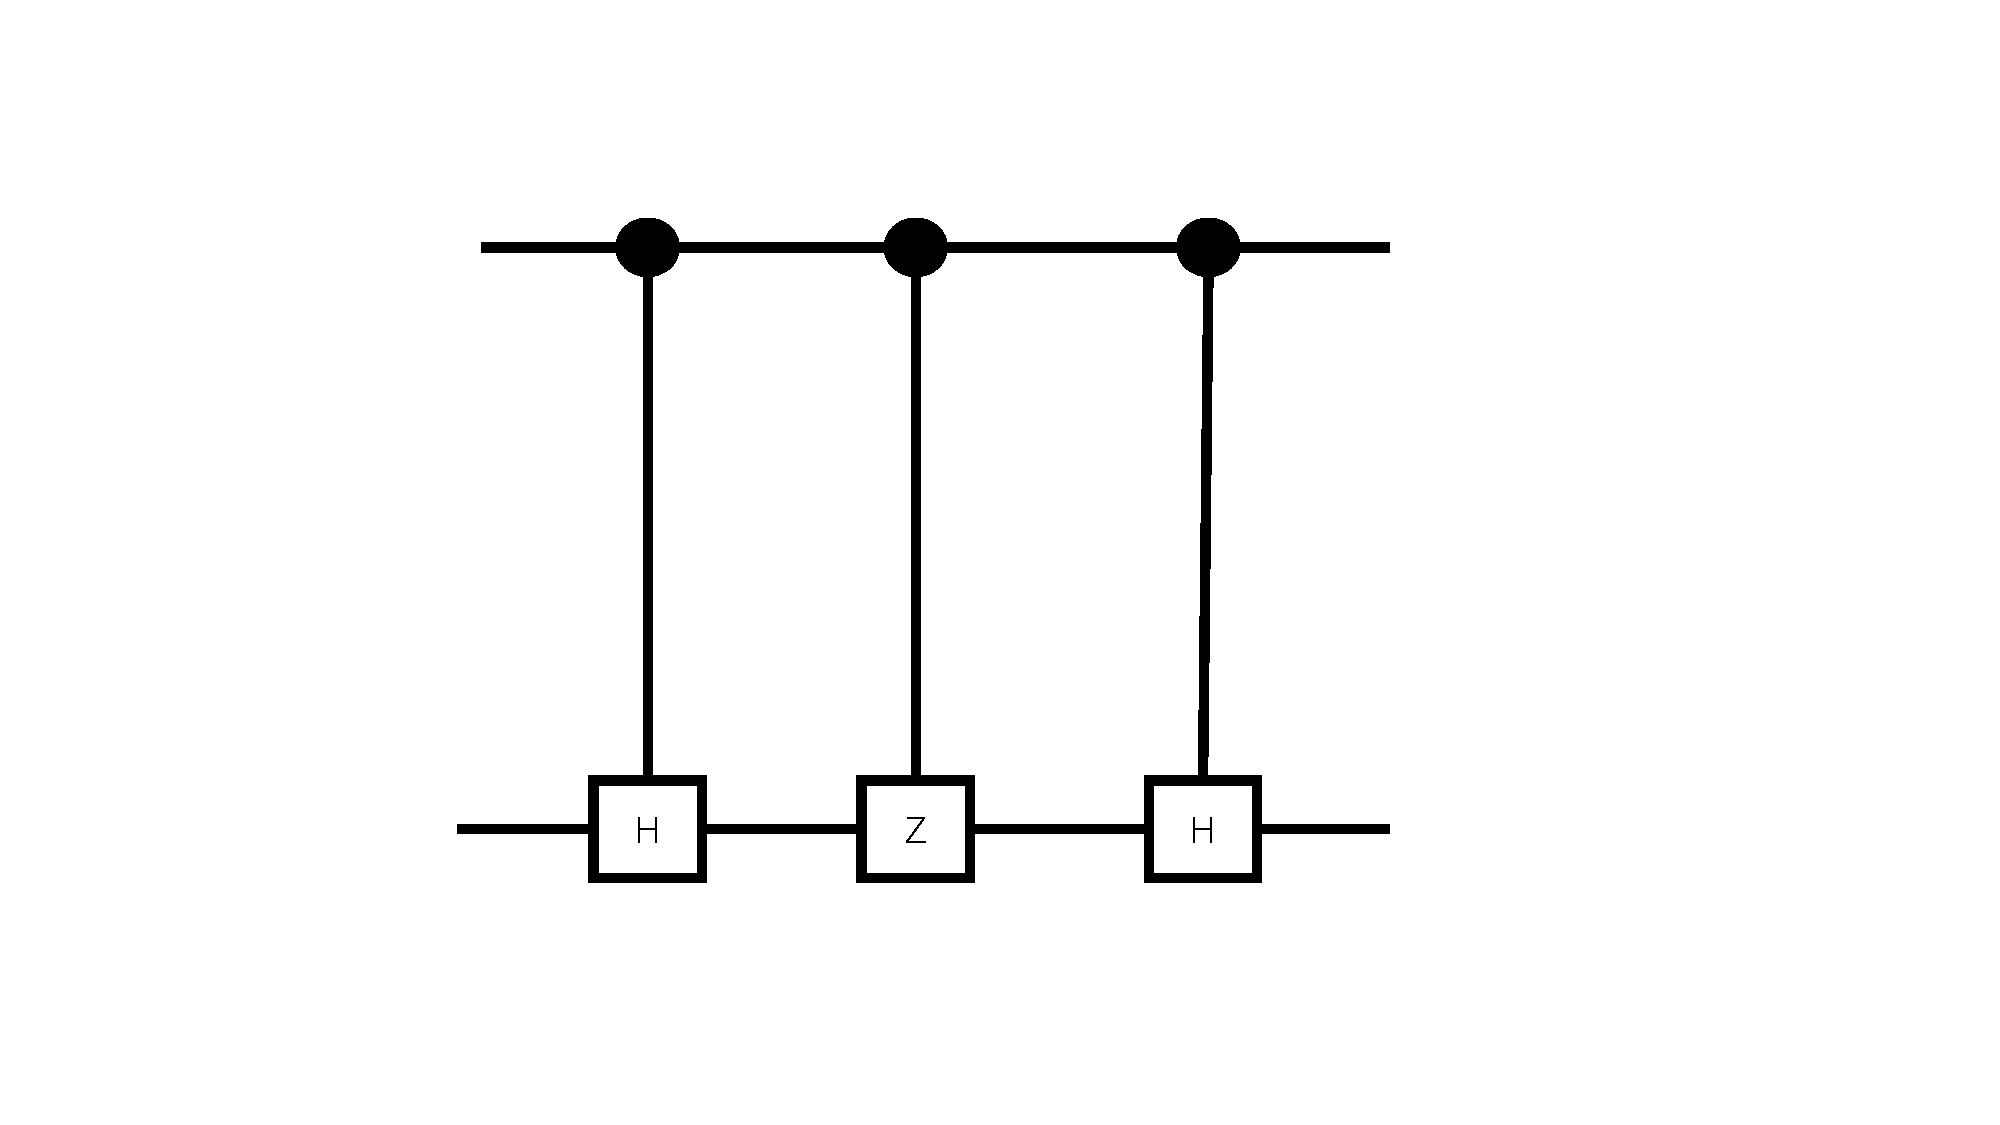
\includegraphics[width=0.7\textwidth]{circuit.pdf}
              \caption{c-X circuit}
          \end{figure}



\end{enumerate}
\end{document}
